%%%%%%%%%%%%%%%%%%%%%%%%%%%%%%%%%%%%%%%%%%%%%%%%%%%%%%%%%%


% Electric Field of Line Charge in TikZ
% https://latexdraw.com
% 16/05/2020, 16:16

\documentclass[border=0.2cm]{standalone}

\usepackage[dvipsnames]{xcolor}
\usepackage{tikz}
\usetikzlibrary{ decorations.markings}


\begin{document}

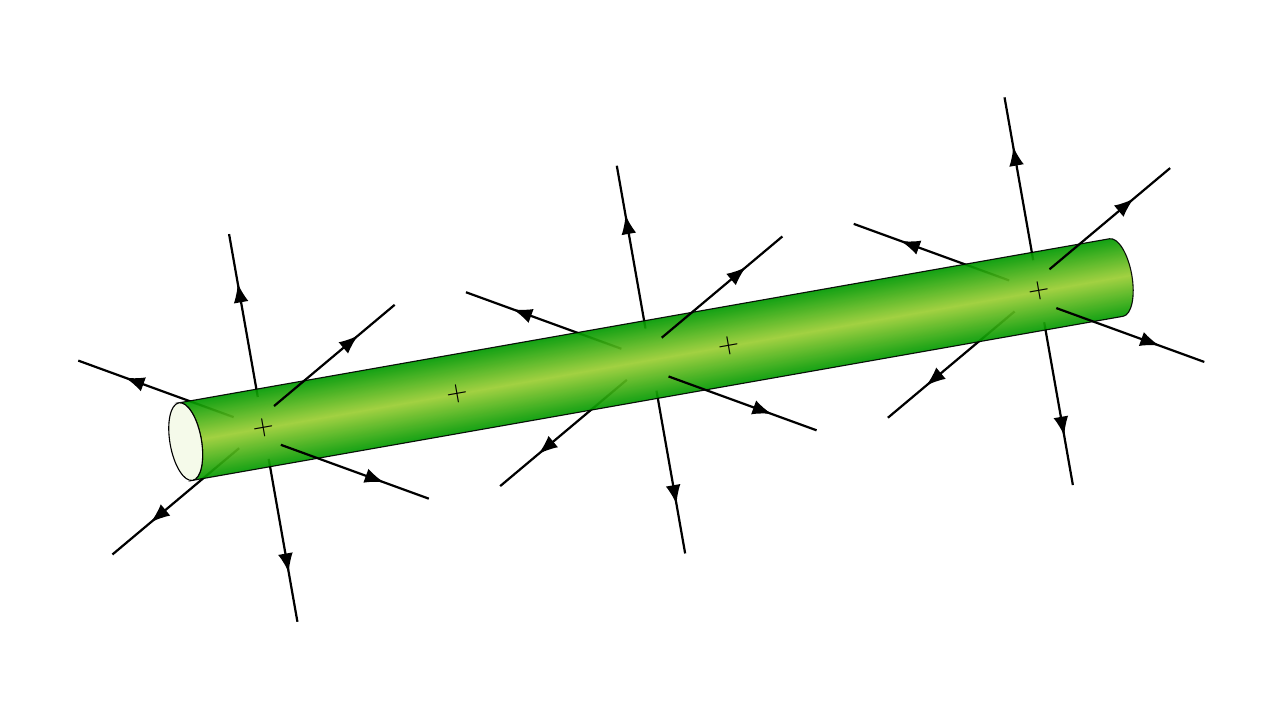
\begin{tikzpicture}
[decoration={markings, 
	mark= at position 0.7 with {\arrow[line width=0.5mm]{latex}}}
] 

% Solve rotation issue
\draw[white] (-2,-3) rectangle (13.5,5.25);

% Rotate the illustration
\begin{scope}[transform canvas={rotate=10}]

% Electric Field (arrows of back layer) 
\foreach \j in{1,6,11}
{
    \begin{scope}[xshift=\j cm]
        \foreach \angle in {90,150,210,270} 
        {
            \draw[thick,postaction={decorate}] (\angle:0.4) -- (\angle:2.5);
        }
    \end{scope}
}
   
% Cylindrical shape
\draw [top color=OliveGreen,
			bottom color=OliveGreen,
			middle color=YellowGreen,
			opacity=0.92] (0,-0.5) -- ++(12,0) 
	arc(-90:90:0.2 and 0.5) -- ++(-12,0) 
	arc(90:-90:0.2 and 0.5)--cycle;

\draw[fill=YellowGreen!10] (0,0) ellipse(0.2 and 0.5);

% Electric charge
\foreach \j in {1,3.5,7,11} 
{
	\node at (\j,0){$+$};
}

% Electric Field (arrows of front layer) 
\foreach \j in {0.75,5.75,10.75}
{
    \begin{scope}[xshift=\j cm]
        \foreach \angle in {-30,30} 
        {
            \draw[thick,postaction={decorate}] (\angle:0.5) -- (\angle:2.5);
        }
    \end{scope}
}
\end{scope} % end scope of the illustration rotation

\end{tikzpicture}

\end{document}
